\subsection{Performance measure of compare operations and event redirection - DPDK}
In this subsection, the performance measure of compare operations and event redirection with bridged virtual machines on EVS DPDK is presented. The set up is similar to the set up in section 5.5.3, except for the rule installed. The operation in consideration is denoted as:

The operation supported by Greater than or equal to operator is denoted by:
\begin{equation}D(e.t  \wedge (e.a_1 <= value) \quad | \quad stream, \end{equation}
where \textit{D} is the detect operation; \newline
\textit{e.t} is the event type; \newline
\textit{e.a1} is the first event attribute; \newline
\textit{value} is the integer value to be compared with; \newline
| denotes the redirect operation; \newline
and \textit{stream} is the logical stream to which the detected event is redirected to. \newline \newline

The controller rule corresponding to this operation that is installed in EVS  is:

\begin{lstlisting}[language=json,firstnumber=1]
{
"dpid": 178974088016461,
"table_id": 0,
"priority": 11112,
"flags": 1,
"match":{
"dl_type":0x0800,
"nw_proto":17,
"nw_src":"10.1.1.1",
"nw_dst":"10.1.1.3",
"tp_dst":9877,
"e_type":"TEST",
},
"actions":[{
"type":"set_nw_dst",
"nw_dst": 10.1.1.2
},
{
"type":"set_dl_dst",
"dl_dst": 00:00:00:00:00:02
},
{
"type":"SET_MAX",
"val": 100
}
]
}
http://localhost:8080/stats/flowentry/add \end{lstlisting}

From the perspective of an event query language, the above rule can be expressed as:

\begin{verbatim}
INSERT INTO NEWTEMPSTREAM
SELECT * FROM TEMPSTREAM 
WHERE DEVICE_1.VALUE <=100
\end{verbatim}

\begin{figure}[H]
	\centering
	\caption{Performance of compare operation and event redirection in bridged virtual machines}
	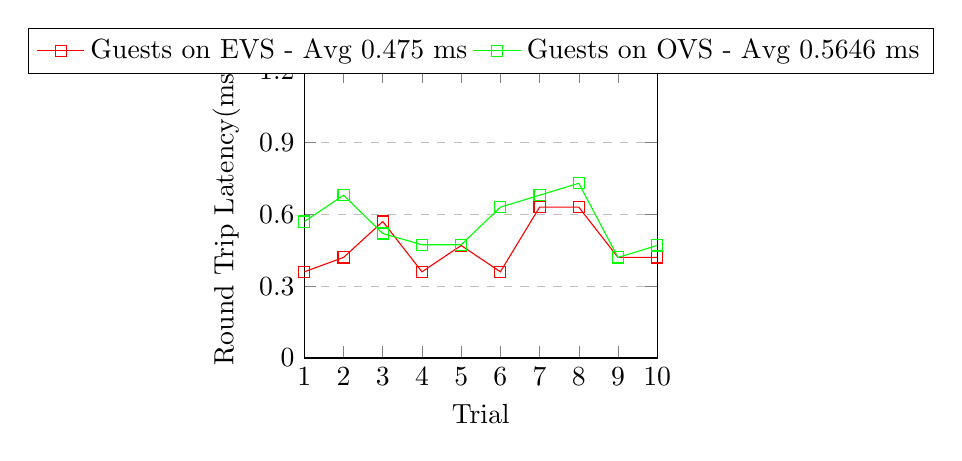
\begin{tikzpicture} [baseline=(current axis.outer east)]
	\begin{axis}[
	width=0.5\textwidth,
	xlabel={Trial},
	ylabel={Round Trip Latency(ms)},
	xmin=1, xmax=10,
	ymin=0.00, ymax=1.2,
	xtick={1,2,3,4,5,6,7,8,9,10},
	ytick={0.00,0.30,0.60,0.90,1.2},
	legend pos=north west,
	ymajorgrids=true,
	grid style=dashed,
	legend style={at={(0.5,1.15)},anchor=north}, legend columns=-1
	]
	\addplot[
	color=red,
	mark=square,
	]
	coordinates {
		(1,0.36)
		(2,0.42)
		(3,0.57)
		(4,0.36)
		(5,0.47)
		(6,0.36)
		(7,0.63)
		(8,0.63)
		(9,0.42)
		(10,0.42)  
		
	};
	\addlegendentry{Guests on EVS - Avg 0.475 ms}
	\addplot[
	color=green,
	mark=square,
	]
	coordinates {
		(1,0.57)
		(2,0.68)
		(3,0.52)
		(4,0.473)
		(5,0.473)
		(6,0.63)
		(7,0.68)
		(8,0.73)
		(9,0.42)
		(10,0.47)
		
	};
	\addlegendentry{Guests on OVS - Avg 0.5646 ms}
	
	
	\end{axis}
	\end{tikzpicture}
\end{figure}

As plotted in the graphs in figure 5.19, for compare operations with disabled megaflow cache, the point-to-point latency in case of the EVS bridge model is slightly lower than while having an application broker in a standard OVS bridge. The results seen are similar to the plot in figure 5.18.
